% Options for packages loaded elsewhere
\PassOptionsToPackage{unicode}{hyperref}
\PassOptionsToPackage{hyphens}{url}
%
\documentclass[
]{article}
\usepackage{lmodern}
\usepackage{amssymb,amsmath}
\usepackage{ifxetex,ifluatex}
\ifnum 0\ifxetex 1\fi\ifluatex 1\fi=0 % if pdftex
  \usepackage[T1]{fontenc}
  \usepackage[utf8]{inputenc}
  \usepackage{textcomp} % provide euro and other symbols
\else % if luatex or xetex
  \usepackage{unicode-math}
  \defaultfontfeatures{Scale=MatchLowercase}
  \defaultfontfeatures[\rmfamily]{Ligatures=TeX,Scale=1}
\fi
% Use upquote if available, for straight quotes in verbatim environments
\IfFileExists{upquote.sty}{\usepackage{upquote}}{}
\IfFileExists{microtype.sty}{% use microtype if available
  \usepackage[]{microtype}
  \UseMicrotypeSet[protrusion]{basicmath} % disable protrusion for tt fonts
}{}
\makeatletter
\@ifundefined{KOMAClassName}{% if non-KOMA class
  \IfFileExists{parskip.sty}{%
    \usepackage{parskip}
  }{% else
    \setlength{\parindent}{0pt}
    \setlength{\parskip}{6pt plus 2pt minus 1pt}}
}{% if KOMA class
  \KOMAoptions{parskip=half}}
\makeatother
\usepackage{xcolor}
\IfFileExists{xurl.sty}{\usepackage{xurl}}{} % add URL line breaks if available
\IfFileExists{bookmark.sty}{\usepackage{bookmark}}{\usepackage{hyperref}}
\hypersetup{
  pdftitle={P8106 Final Project},
  pdfauthor={Phoebe Mo(km3624), Stella Li(cl4043), Yihan Feng(yf2555)},
  hidelinks,
  pdfcreator={LaTeX via pandoc}}
\urlstyle{same} % disable monospaced font for URLs
\usepackage[margin=1in]{geometry}
\usepackage{color}
\usepackage{fancyvrb}
\newcommand{\VerbBar}{|}
\newcommand{\VERB}{\Verb[commandchars=\\\{\}]}
\DefineVerbatimEnvironment{Highlighting}{Verbatim}{commandchars=\\\{\}}
% Add ',fontsize=\small' for more characters per line
\usepackage{framed}
\definecolor{shadecolor}{RGB}{248,248,248}
\newenvironment{Shaded}{\begin{snugshade}}{\end{snugshade}}
\newcommand{\AlertTok}[1]{\textcolor[rgb]{0.94,0.16,0.16}{#1}}
\newcommand{\AnnotationTok}[1]{\textcolor[rgb]{0.56,0.35,0.01}{\textbf{\textit{#1}}}}
\newcommand{\AttributeTok}[1]{\textcolor[rgb]{0.77,0.63,0.00}{#1}}
\newcommand{\BaseNTok}[1]{\textcolor[rgb]{0.00,0.00,0.81}{#1}}
\newcommand{\BuiltInTok}[1]{#1}
\newcommand{\CharTok}[1]{\textcolor[rgb]{0.31,0.60,0.02}{#1}}
\newcommand{\CommentTok}[1]{\textcolor[rgb]{0.56,0.35,0.01}{\textit{#1}}}
\newcommand{\CommentVarTok}[1]{\textcolor[rgb]{0.56,0.35,0.01}{\textbf{\textit{#1}}}}
\newcommand{\ConstantTok}[1]{\textcolor[rgb]{0.00,0.00,0.00}{#1}}
\newcommand{\ControlFlowTok}[1]{\textcolor[rgb]{0.13,0.29,0.53}{\textbf{#1}}}
\newcommand{\DataTypeTok}[1]{\textcolor[rgb]{0.13,0.29,0.53}{#1}}
\newcommand{\DecValTok}[1]{\textcolor[rgb]{0.00,0.00,0.81}{#1}}
\newcommand{\DocumentationTok}[1]{\textcolor[rgb]{0.56,0.35,0.01}{\textbf{\textit{#1}}}}
\newcommand{\ErrorTok}[1]{\textcolor[rgb]{0.64,0.00,0.00}{\textbf{#1}}}
\newcommand{\ExtensionTok}[1]{#1}
\newcommand{\FloatTok}[1]{\textcolor[rgb]{0.00,0.00,0.81}{#1}}
\newcommand{\FunctionTok}[1]{\textcolor[rgb]{0.00,0.00,0.00}{#1}}
\newcommand{\ImportTok}[1]{#1}
\newcommand{\InformationTok}[1]{\textcolor[rgb]{0.56,0.35,0.01}{\textbf{\textit{#1}}}}
\newcommand{\KeywordTok}[1]{\textcolor[rgb]{0.13,0.29,0.53}{\textbf{#1}}}
\newcommand{\NormalTok}[1]{#1}
\newcommand{\OperatorTok}[1]{\textcolor[rgb]{0.81,0.36,0.00}{\textbf{#1}}}
\newcommand{\OtherTok}[1]{\textcolor[rgb]{0.56,0.35,0.01}{#1}}
\newcommand{\PreprocessorTok}[1]{\textcolor[rgb]{0.56,0.35,0.01}{\textit{#1}}}
\newcommand{\RegionMarkerTok}[1]{#1}
\newcommand{\SpecialCharTok}[1]{\textcolor[rgb]{0.00,0.00,0.00}{#1}}
\newcommand{\SpecialStringTok}[1]{\textcolor[rgb]{0.31,0.60,0.02}{#1}}
\newcommand{\StringTok}[1]{\textcolor[rgb]{0.31,0.60,0.02}{#1}}
\newcommand{\VariableTok}[1]{\textcolor[rgb]{0.00,0.00,0.00}{#1}}
\newcommand{\VerbatimStringTok}[1]{\textcolor[rgb]{0.31,0.60,0.02}{#1}}
\newcommand{\WarningTok}[1]{\textcolor[rgb]{0.56,0.35,0.01}{\textbf{\textit{#1}}}}
\usepackage{graphicx,grffile}
\makeatletter
\def\maxwidth{\ifdim\Gin@nat@width>\linewidth\linewidth\else\Gin@nat@width\fi}
\def\maxheight{\ifdim\Gin@nat@height>\textheight\textheight\else\Gin@nat@height\fi}
\makeatother
% Scale images if necessary, so that they will not overflow the page
% margins by default, and it is still possible to overwrite the defaults
% using explicit options in \includegraphics[width, height, ...]{}
\setkeys{Gin}{width=\maxwidth,height=\maxheight,keepaspectratio}
% Set default figure placement to htbp
\makeatletter
\def\fps@figure{htbp}
\makeatother
\setlength{\emergencystretch}{3em} % prevent overfull lines
\providecommand{\tightlist}{%
  \setlength{\itemsep}{0pt}\setlength{\parskip}{0pt}}
\setcounter{secnumdepth}{-\maxdimen} % remove section numbering
\usepackage{booktabs}
\usepackage{longtable}
\usepackage{array}
\usepackage{multirow}
\usepackage{wrapfig}
\usepackage{float}
\usepackage{colortbl}
\usepackage{pdflscape}
\usepackage{tabu}
\usepackage{threeparttable}
\usepackage{threeparttablex}
\usepackage[normalem]{ulem}
\usepackage{makecell}
\usepackage{xcolor}

\title{P8106 Final Project}
\author{Phoebe Mo(km3624), Stella Li(cl4043), Yihan Feng(yf2555)}
\date{5/7/2021}

\begin{document}
\maketitle

\hypertarget{introduction}{%
\section{1. INTRODUCTION}\label{introduction}}

\hypertarget{motivation-and-objective}{%
\subsection{1.1 Motivation and
Objective}\label{motivation-and-objective}}

Pokemon are fictional creatures, which can be captured by players and
trained to battle each other in the augmented reality game Pokémon Go!.
In this project, we use a dataset from Kaggle that contains different
attributes and catch rates for 721 unique Pokemons. We try to understand
the relationship between Pokemons' different attributes and their
respective catch rates. Here are some questions we want to answer: Which
predictor(s) play important roles in predicting catch rates? Which type
of model (linear or non-linear) serves as a better method to predict the
catch rate?

\hypertarget{data-preparation-and-cleaning}{%
\subsection{1.2 Data Preparation and
Cleaning}\label{data-preparation-and-cleaning}}

The original dataset has 20 predictors such as HP, and the outcome
`catch\_rate'. After cleaning the names of these variables, I did the
following steps to clean the data:

1.2.1 Notice that `type\_2' and `egg\_group\_2' are indicators of if a
pokemon has a second type or belongs to a second egg group. The `Null'
values in the data means the pokemon does not has the second type/group,
so I changed them into ``none'' to make them as a category to be
meaningful;

1.2.2 The `generation' predictor is originally a numeric type, but it
has only 6 integer values, so I decided to mutate it to be categorical;

1.2.3. Irrelevant variables `number' and `name' are dropped. `total',
which is the total base battle statistic for each pokemon, is calculated
and reflected in other battle attributes such as `hp' and `attack'. So I
dropped it to avoid intercollinearity. Later, after plotting the
correlation map, I found `weight\_kg' and `height\_m' has relatively
high correlation(correlation plot is shown in section 2). After
consideration, I chose to drop `height\_m' since it may has less effect
on catch rate compared to `weight\_kg'. `has\_gender' is also dropped
because all values are ``TRUE''.

\hypertarget{exploratory-analysis-visualization}{%
\section{2. Exploratory Analysis /
Visualization}\label{exploratory-analysis-visualization}}

After plotting scatter plots for numerical predictors and boxplots for
categorical predictors, significant trends were not observed in
different types, egg groups, body\_styles or colors. However, the battle
attributes: `hp', `attack', `defense', `sp\_atk', `sp\_def', and `speed'
seem to have a negative association with catch rate. While
\texttt{total} doesn't have an obvious trend. Therefore, we decided to
keep specific battle features for analysis.

The `weight\_kg' also seems to have negative association with catch
rate. And the pokemons that are legendary have significantly lower catch
rates. Below are some selected visualizations:

\includegraphics{DS_FinalProject_files/figure-latex/unnamed-chunk-3-1.pdf}
\includegraphics{DS_FinalProject_files/figure-latex/unnamed-chunk-3-2.pdf}
\includegraphics{DS_FinalProject_files/figure-latex/unnamed-chunk-3-3.pdf}

\hypertarget{models}{%
\section{3. Models}\label{models}}

The dataset for analysis contains 644 samples and 18 predictors:

\begin{itemize}
\tightlist
\item
  \texttt{type\_1}: primary type
\item
  \texttt{typw\_2}: second type, in case the Pokémon has it
\item
  \texttt{hp}: health point
\item
  \texttt{attack}: base attack
\item
  \texttt{defense}: base defense
\item
  \texttt{sp\_atk}: attack speed
\item
  \texttt{sp\_def}: defense speed
\item
  \texttt{speed}: base speed
\item
  \texttt{generation}: number of the generation when the Pokémon was
  introduced
\item
  \texttt{is\_legendary}: Boolean that indicates whether the Pokémon is
  Legendary or not
\item
  \texttt{color}: color of the Pokémon according to the Pokédex
\item
  \texttt{pr\_male}: probability of being a male Pokemon
\item
  \texttt{egg\_group\_1}: egg group of the Pokémon
\item
  \texttt{egg\_group\_2}: second egg group of the Pokémon, in case it
  has two
\item
  \texttt{has\_mega\_evolution}: Boolean that indicates whether the
  Pokémon is able to Mega-evolve or not
\item
  \texttt{height\_m}: height of the Pokémon, in meters
\item
  \texttt{weight\_kg}: weight of the Pokémon, in kilograms
\item
  \texttt{body\_style}: body style of the Pokémon according to the
  Pokédex
\item
  \texttt{catch\_rate}: the response (on 0 - 255 scale)
\end{itemize}

The dataset is split into 75:25 training to test dataset. Based on our
midterm project, We include GAM model, since it has a dominant
performance among other methods(e.g.~lda, qda, nb, lasso, ridge\ldots),
as a competitive model for predicting the catch rate. We also choose
Boosting, Random Forest, Bagging, and Support Vector Machine models to
train the data with cross validation. RMSE is used to compare and choose
the final model. Finally, we use clustering to have a better
visualization of pokemons that have similar attributes and to see if
significant relationship between combat attributes and catch rate can be
found.

\hypertarget{gam}{%
\subsection{3.1 GAM}\label{gam}}

Based on the visualization plots, we can see that some continuous
variables have curve-like trend in the right tail. In this case, I
consider using GAM model in order to include this trend into the
analysis. For such predictors, I allow GAM to make it non-parametric
smoothing term. GCV is used to choose the degree of freedom for the
model.

After fitting, it is observed that the smooth terms of `hp', `attack',
`defense', `sp\_atk', `speed', and the coefficients of `type\_1Poison',
`type\_2Water', `generation3', `pr\_male', `egg\_group\_1Undiscovered',
`body\_stylemultiple\_bodies', are significant. These result greatly
coincides with the ones given by previous model.

\hypertarget{bagging-boosting-random-forest}{%
\subsection{3.2 Bagging, Boosting, Random
Forest}\label{bagging-boosting-random-forest}}

We decide to use tree-based ensemble methods for regression. The
function \texttt{randomForest()} implements Breiman's random forest
algorithm for classification and regression, since our data is high
dimensional, we also used function \texttt{ranger()} for training the
random forest model. \newline Since Random Forest does not have any
underlying models, so it does not have assumptions, other than there is
no multicollinearity among the variables. \newline For bagging, we used
all 18 predictors for training.

Boosting primarily aims at reducing bias and variance. For boosting, we
first did a grid search using \texttt{caret}. We then used the fast
implementation of random forest when tuning the model and tuned the gbm
model based on its result.

\hypertarget{svm}{%
\subsection{3.3 SVM}\label{svm}}

In SVM, we want to find a separating hyperplane that maximizes the gap
between classes to optimally predict the outcome. Support Vector Machine
with both linear and radial kernel is used to train the data. The tuning
parameter epsilon(trade-off between correct classification and
maximization of the gap) and gamma(how non-linear the fit could be) are
tuned given a suitable range of numbers in the function.

\hypertarget{clustering}{%
\subsection{3.4 Clustering}\label{clustering}}

In order to have a better visualization of the relationship between the
pokemon and their different attributes, we use both k-means clustering
and hierarchical clustering to group similar pokemons together. Here, we
use only numerical variables. As can see from k-means clustering (Figure
4), we use the optimal number of clusters = 3 and use Euclidean distance
to decide the similarity. From the plot briefly, cluster 1 tends to has
lower hp, cluster 2 has lower catch\_rate, and cluster 3 has relatively
higher weight and defense. \newline For the hierarchical clustering, we
use complete linkage(maximal inter-cluster dissimilarity) and euclidean
distance. Since hierarchical clustering provides us all the possible
combinations of clusters, to visualize, we made a heat map to see how
all the variables vary for each observation. From the heat map (Figure
5), we found pokemons that have higher hp, height, and weight tend to
have lower catch\_rate, whereas those which have relatively low combat
attributes tend to have higher catch\_rate.

\hypertarget{variable-importance-and-clustering-results}{%
\subsection{3.5 Variable Importance and Clustering
Results}\label{variable-importance-and-clustering-results}}

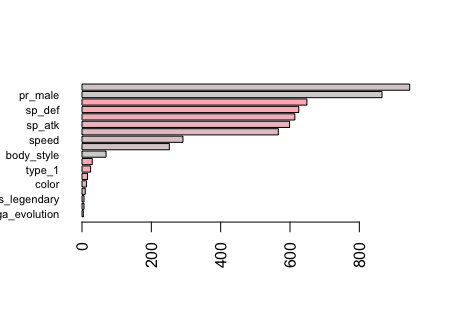
\includegraphics[width=6.25in]{./plot/rf_vi}
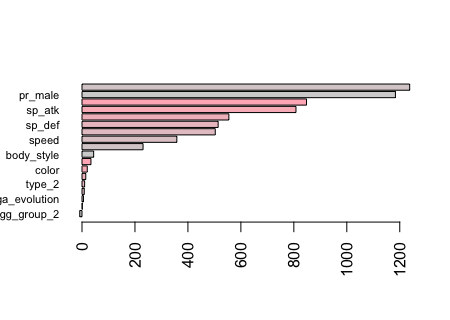
\includegraphics[width=6.25in]{./plot/bag_vi}
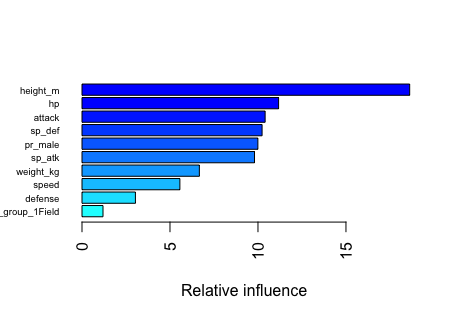
\includegraphics[width=6.25in]{./plot/boost_vi}
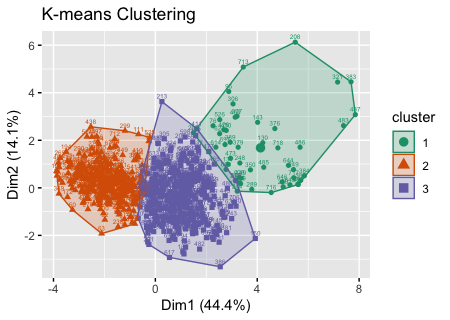
\includegraphics[width=6.25in]{./plot/k-mean-cluster-plot}
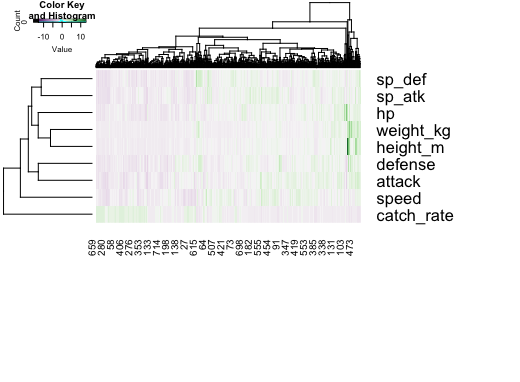
\includegraphics[width=7.22in]{./plot/hc-heatmap}

\hypertarget{final-model-and-visualization}{%
\subsection{3.6 Final Model and
Visualization}\label{final-model-and-visualization}}

\hypertarget{conclusions}{%
\section{4. Conclusions}\label{conclusions}}

4.1 According to the Cross-Validation RMSE (Table 1), Bagging has the
lowest RMSE ≈ 18.91, meaning among these models, Bagging is the best
candidate to predict the catch rate. Although we picked GAM model before
having these new models, it seems like all the new models, except for
SVM (using linear kernel), have better performance than the GAM model.
Random Forest and boosting also have very good performance.

4.2 The outcomes given by our models and clustering coincide with our
expectation and initial visualization that, pokemons which have better
combat attributes(e.g.~attack, defense\ldots) have a lower catch rate.
But we did not expect that the probability of having male pokemons may
also affect the catch rate, which is quite surprising.

Also, we expected to see random forest model may be the best candidate
to predict catch rate because it helps improve bagging by decorrelating
the trees, but in fact, Bagging model performs the best in out project.

4.3 Variable Importance (Figure 6)

\begin{enumerate}
\def\labelenumi{\arabic{enumi}.}
\tightlist
\item
  The top 5 important variables resulted from random forest is:
\end{enumerate}

\begin{itemize}
\tightlist
\item
  pr\_male
\item
  sp\_def
\item
  sp\_atk
\item
  speed
\item
  body\_style
\end{itemize}

\begin{enumerate}
\def\labelenumi{\arabic{enumi}.}
\setcounter{enumi}{1}
\tightlist
\item
  The top 5 important variables resulted from bagging is:
\end{enumerate}

\begin{itemize}
\tightlist
\item
  pr\_male
\item
  sp\_atk
\item
  sp\_def
\item
  speed
\item
  body\_style
\end{itemize}

\begin{enumerate}
\def\labelenumi{\arabic{enumi}.}
\setcounter{enumi}{2}
\tightlist
\item
  The top 5 important variables resulted from boosting is:
\end{enumerate}

\begin{itemize}
\tightlist
\item
  height\_m
\item
  hp
\item
  attack
\item
  sp\_def
\item
  pr\_male
\end{itemize}

Based on the 3 models, important variables are speed of defense
(sp\_def), probability of male Pokemon (pr\_male), speed, speed of
attack (sp\_atk), and body style.

4.4 Clustering We found Pokemons that have higher hp, height, and weight
tend to have lower catch\_rate, whereas those which have relatively low
combat attributes tend to have higher catch\_rate.

\hypertarget{limitations}{%
\section{5. Limitations}\label{limitations}}

5.1 The GAM model does not truly select the tuning parameter and do the
model training, therefore this may be the limitation of the GAM model.
However, since it has the smallest training RMSE, we still decide to
choose it as our best method for the prediction in this project.

5.2 For the k-means clustering, since we need to decide k ourselves,
there is no reference for us to decide which k is better. So the
manually selected k and the given visualization may not be the best
presentation.

5.3 There are no specific assumptions for the Random Forest model.

\hypertarget{appendix}{%
\section{Appendix}\label{appendix}}

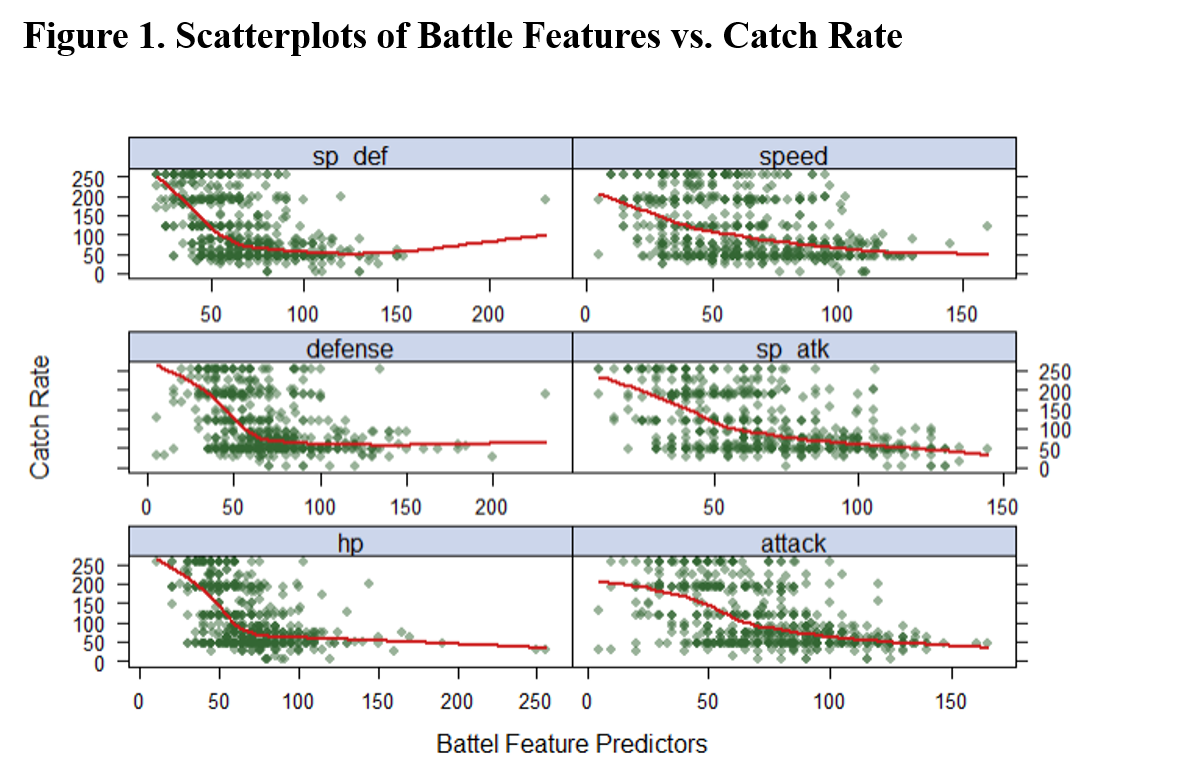
\includegraphics{anno_fig/fig1.png}

\begin{Shaded}
\begin{Highlighting}[]
\NormalTok{total.plot}
\end{Highlighting}
\end{Shaded}

\includegraphics{DS_FinalProject_files/figure-latex/unnamed-chunk-13-1.pdf}

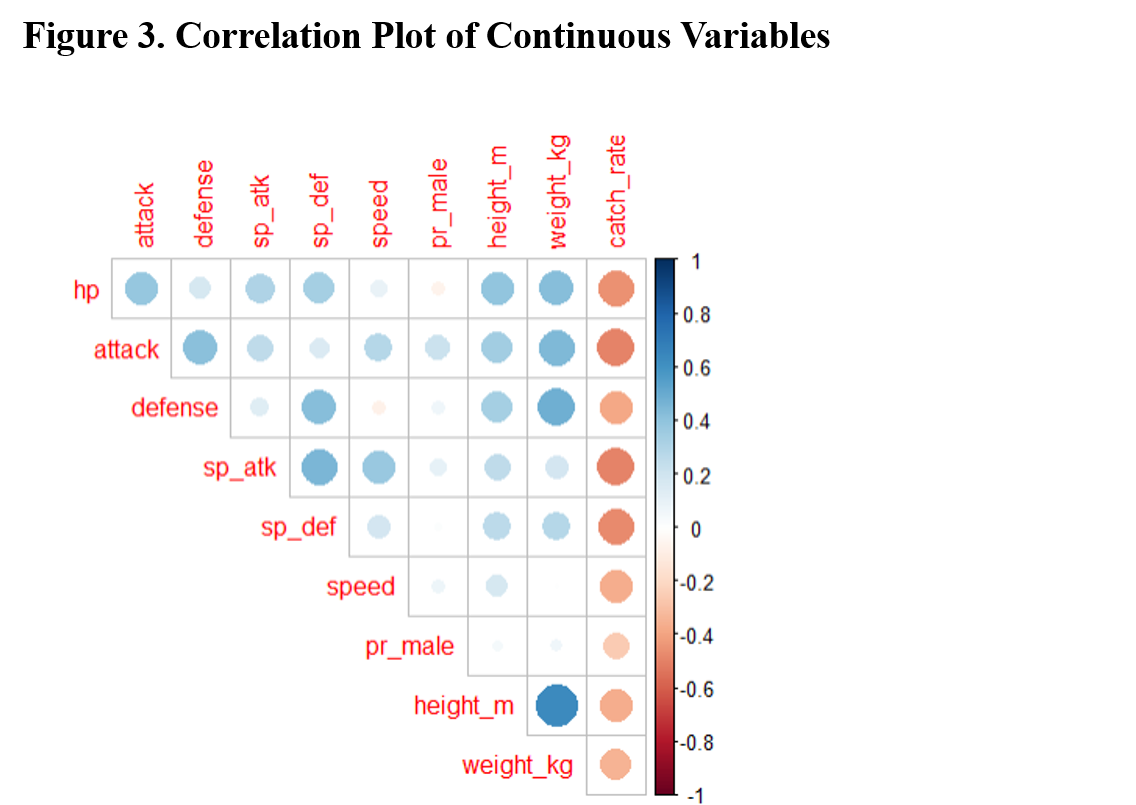
\includegraphics{anno_fig/fig3.png} 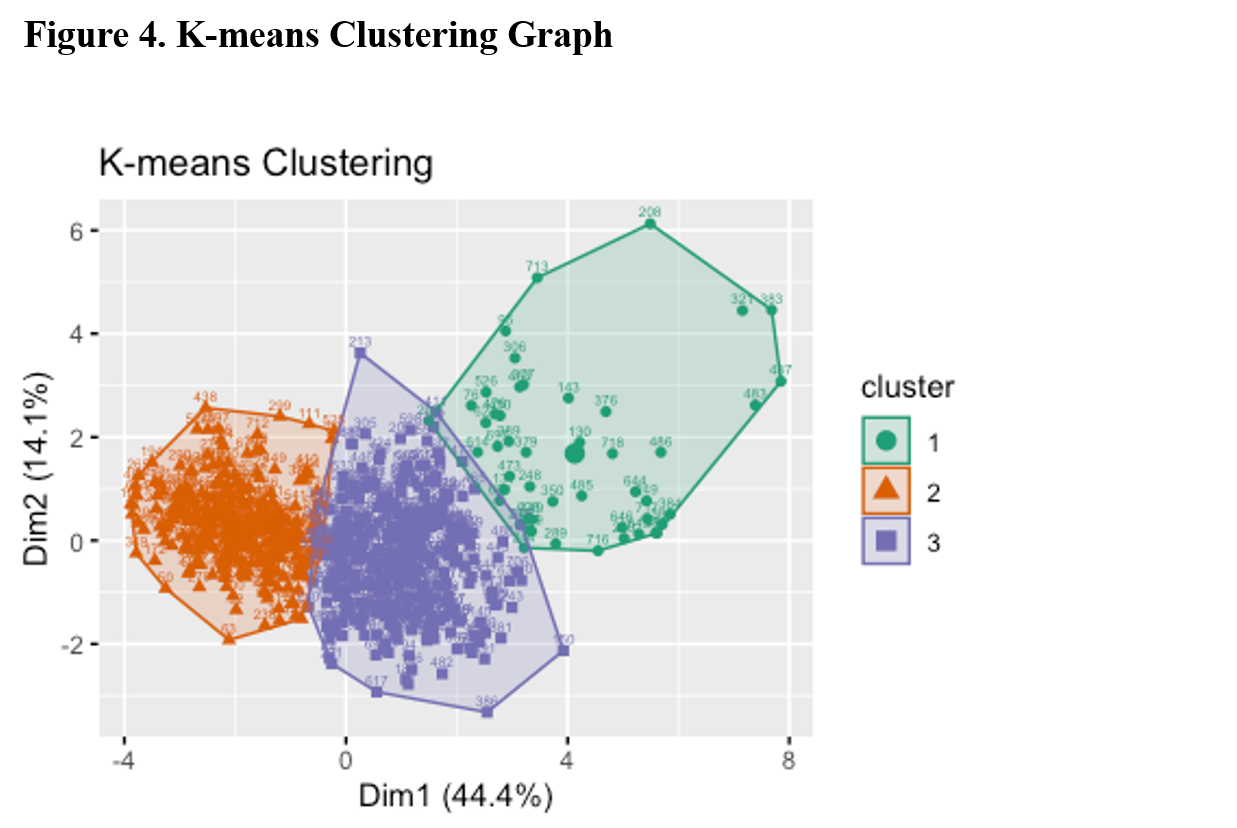
\includegraphics{anno_fig/fig4.png}
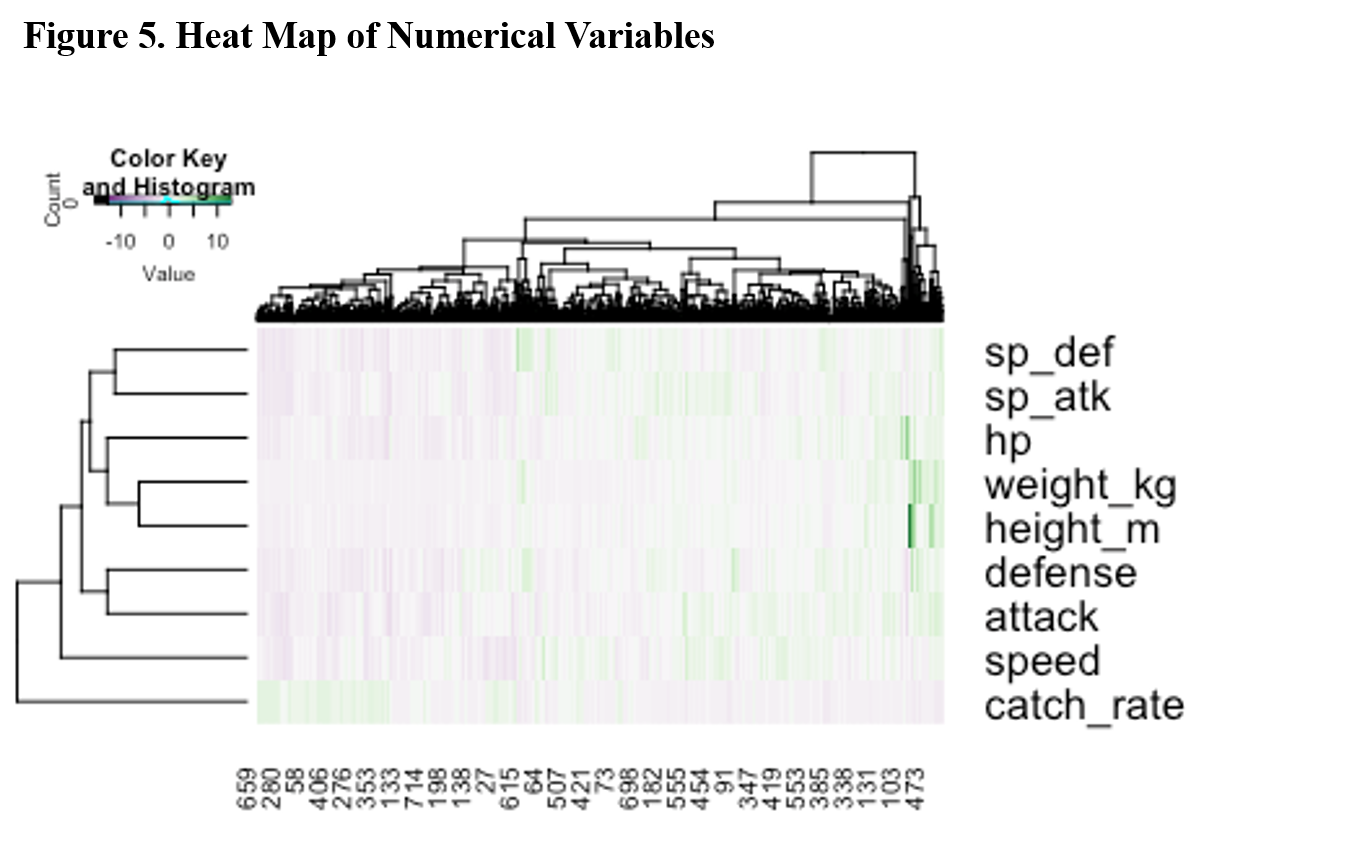
\includegraphics{anno_fig/fig5.png} 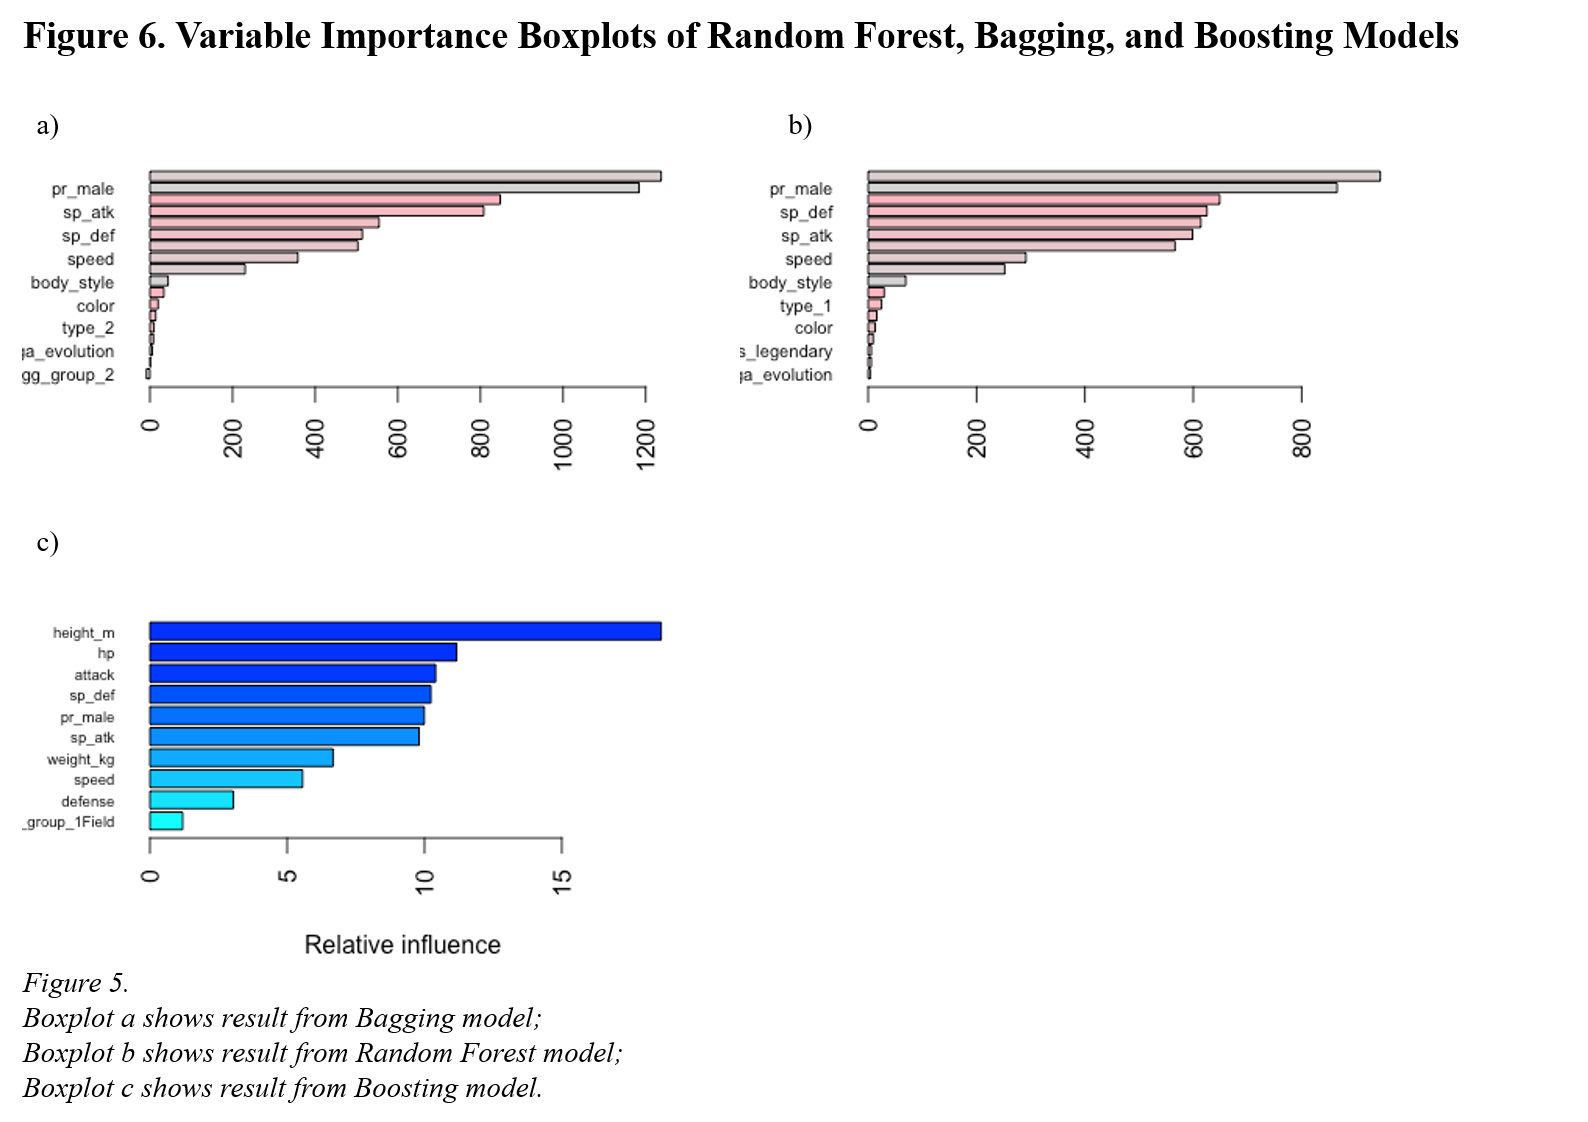
\includegraphics{anno_fig/fig6.png}

\begin{Shaded}
\begin{Highlighting}[]
\NormalTok{final_rmse1}
\end{Highlighting}
\end{Shaded}

\begin{table}

\caption{\label{tab:unnamed-chunk-12}Table 1. Cross Validation RMSE Table}
\centering
\begin{tabular}[t]{l|r}
\hline
Model & RMSE\\
\hline
GAM & 42.11\\
\hline
Boosting & 19.88\\
\hline
Random Forest & 19.76\\
\hline
Bagging & 18.91\\
\hline
SVM (linear) & 44.79\\
\hline
SVM (radial) & 35.27\\
\hline
\end{tabular}
\end{table}

\end{document}
